\documentclass[12pt]{extarticle}
\setlength{\columnsep}{1cm}
\usepackage[utf8]{inputenc}
\usepackage[margin=.5in]{geometry}
\usepackage{amsmath}
\usepackage{amsfonts}
\usepackage{amssymb}
\usepackage{hyperref}
\usepackage{listings}
\usepackage{appendix}
\usepackage{graphicx}
\graphicspath{ {graphs/} }

% \usepackage{listings}
\usepackage{color}
\usepackage{multicol}

\definecolor{dkgreen}{rgb}{0,0.6,0}
\definecolor{gray}{rgb}{0.5,0.5,0.5}
\definecolor{mauve}{rgb}{0.58,0,0.82}

\lstset{frame=tb,
  language=Java,
  aboveskip=3mm,
  belowskip=3mm,
  showstringspaces=false,
  columns=flexible,
  basicstyle={\small\ttfamily},
  numbers=none,
  numberstyle=\tiny\color{gray},
  keywordstyle=\color{blue},
  commentstyle=\color{dkgreen},
  stringstyle=\color{mauve},
  breaklines=true,
  breakatwhitespace=true,
  tabsize=3
}

\newcommand{\hwname}{Jules Sang}
\newcommand{\hwemail}{jules.sang@grenoble-inp.org}
\renewcommand{\familydefault}{\sfdefault}

\title{Efficient Algorithms - Step 4}
\author{\hwname \\ \hwemail}

\begin{document}
\maketitle
\tableofcontents

\newpage
\begin{multicols}{2}
\begin{abstract}
  In this paper, the efficiency of different parsing algorithms is analyzed,
  both for Chomsky normal form grammars and linear grammars.

  First part investigates the parsing of Chomsky normal form grammars with
  (i) a naive top-down algorithm, (ii) a memoization algorithm, and (iii) the
  widely-known Cocke-Younger-Kasami tabulation algorithm.

  Second part investigates linear grammars' parsing with (i) converting linear
  grammars to Chomsky normal form, then applying the Cocke-Younger-Kasami
  algorithm, (ii) adapting the Cocke-Younger-Kasami algorithm to linear grammars.

  Both parts show theorical and empirical views of the algorithms' efficiency.
\end{abstract}

\section*{Introduction}
Parsing is the process of analysing a string of symbols, conforming to the rules
of a formal gramar.
It is a fundamental computer science notion: The parser is one of the main
parts of compilers and interpreters, which describe how programs should be executed by
the machine. Since most modern languages are context-free (and thus expressible
by context-free grammars (see \ref{cfg}), parsers for context-free languages can be
used to check that programs are syntactically correct.
% It is hence important to have the most efficient parsing algorithms.
Developing efficient parsing algorithms for context-free grammars hence allows a faster compilation or
interpretation of programs.

\section{Central notions}
\subsection{Context-free grammar (CFG)} \label{cfg}
Parsers need a set of formal rules in order to interpret the symbols of input
strings, and define syntactic
relations between symbols. This set of formal rules is called a grammar, and
is used to express a language's semantics.
A context-free grammars is a special type of grammar, that can
express most modern programming languages.

\subsubsection{Definition}
A context-free grammar is defined by $G=(N,\Sigma,P,S)$, where:\\
\begin{enumerate}
  \item $N$ is a finite set, $A\in N$ is called a nonterminal element.
  \item $\Sigma$ is a finite set, $N\cap\Sigma=\emptyset$, $\sigma\in\Sigma$ is called a terminal element.
  \item $P:N\rightarrow (N\cup \Sigma)^*$ is a finite set of production rules.
    The ``*'' symbol expresses a multiplicity. Here it means ``the concatenation
    of any number of elements from $N$ and $\Sigma$''.
  \item $S\in N$ is called the starting symbol of $G$.
\end{enumerate}
% $L(G)=\{w\in \Sigma^*|S\Rightarrow^*w\}$ (Where $S \Rightarrow^* w$ means that
% $w$ can be generated from $S$ by using one or multiple rules)
$L(G)=\{w\in \Sigma^*|S$ generates\footnote{Given a production rule
  $A\rightarrow \alpha$, we say that $A$ generates $\alpha$. Given $A\rightarrow
  B$, and $B\rightarrow\alpha$, $A$ generates $\alpha$ by transitivity.} $w\}$
is called the language generated by $G$, and corresponds to the set of
terminal strings that can be generated starting from $S$ with production rules
from $P$.

\paragraph{Example of CFG} 
\begin{align*}
  G&=(N,\Sigma,P,A)\\
  N&=\{A,B\}\\
  \Sigma&=\{\alpha,\beta\}\\
  P&=\{A\rightarrow\alpha B\beta | \alpha, B\rightarrow\beta A\alpha | \beta\}
\end{align*}

For example, $\{\alpha, \alpha\beta\alpha, \alpha\beta\alpha\alpha\}\subset L(G)$


\subsection{Chomsky normal form (CNF) grammars}
A context-free grammar $G$ is said to be in Chomsky normal form if all of its production rules are of the form
\begin{itemize}
\item $A\rightarrow BC$ or
\item $A\rightarrow\alpha$ or
\item $S\rightarrow\epsilon$
\end{itemize}
Where $A,B,C$ are nonterminals, $S$ is the starting symbol of $G$, and $\epsilon$
denotes the empty string. Also,  if $S\rightarrow\epsilon$ is a production
rule of $G$, $S$ may not appear in the right-hand side of any production rule.
Any CFG can be transformed into a CNF grammar, with a size no larger than the square of the initial grammar's size.

\subsection{Linear grammars}\label{sec:linear}
A context-free grammar is said to be linear if there is at most one nonterminal
symbol in the right-hand side of its production rules.

\subsection{Some common algorithmic techniques}
This section presents the main principles of the algorithmic techniques used in this paper.

\subsubsection{Tabulation}
Tabulation is a dynamic programming technique that focuses on building up larger and larger subsolutions to a problem until the target solution has been reached. Each iteration uses the results of the previous ones to compute the solution faster. Tabulation algorithms are bottom-up and iterative by nature.

\paragraph{Example of a tabulation algorithm} Here is how one would use tabulation for computing fibonacci:\\
\begin{lstlisting}
  function fibo(n):
      mem[0] <- 0
      mem[1] <- 1

      for i in 2...n:
          mem[i] = mem[i-1] + mem[i-2]
      
      return mem[n]
\end{lstlisting}

\subsubsection{Memoization}
Memoization is a dynamic programming technique where the result of time-expansive function calls are stored in a data structure, in order to avoid recomputing them if the same inputs occur again. Memoization algorithms are top-down and recursive by nature.

\paragraph{Example of a memoization algorithm} Here is how one would use memoization for computing fibonacci:\\
\begin{lstlisting}
  function fibo(n):
      if n < 2:
          return n

      if mem[n] is null:
          mem[n] = fibo(n-1) + fibo(n-2)
          
      return mem[n]
\end{lstlisting}

\newpage
\section{Parsing algorithms}
\subsection{The Cocke-Younger-Kasami (CYK) algorithm}
The CYK algorithm is a parsing algorithm: in its standard version, the input is
$G$, a context-free
grammar in CNF, and $\alpha$ a string. The output is true if and only if $\alpha\in L(G)$.
It is easy to tweak the algorithm so that it returns the rules of $G$ used for
generating $\alpha$, without additional space or memory costs.

The original version of the CYK algorithm is bottom-up. The two other versions
presented here after are variants.

\subsubsection{Naive top-down implementation}
Let $G$ be the grammar, $\Sigma$ the set of nonterminals symbols of $G$, $P$ the rules of $G$, $\alpha$ the string to parse and $S\in \Sigma$ the starting symbol of $G$.\\
Here is how \textit{parse($S$, $\alpha$)} behaves:
\begin{itemize}
\item If $|\alpha|=1$: Return true if $(S\rightarrow\alpha)\in P$ else return false
\item If $|\alpha|>1$: For each $(S\rightarrow AB)\in P$, and for each possible partition of $\alpha$ into two parts $\beta$ and $\delta$, return true if
both \textit{parse($A$, $\beta$)} and \textit{parse($B$, $\delta$)} return true. If no such combination of $(A,B,\beta,\delta)$ is found, return false
% it is possible to parse both $\beta$ with $A$ as the starting symbol, and $\delta$ with $B$ as the starting symbol. If there is atleast one possibility, return true, else false.
\end{itemize}

This algorithm consists of a recursive enumeration of each applicable rule.

\paragraph{Pseudocode} Here is the pseudocode for naive the top-down implementation:
\begin{lstlisting}
    function naive(G: the grammar, S: the starting symbol, alpha[i, j]: the string):
        if j = 1:
            return G.contains(S -> alpha)

        for each P production rule of G, of the form S -> AB:
            for k = i+1...j-1:
                if naive(G, A, alpha[i, k]) and naive(G, B, alpha[k, j]):
                    return true

        return false
\end{lstlisting}

% TODO: find the complexity
\paragraph{Complexity:}
Note that, depending on the implementation, recursive calls imply a copy of the
considered substring, and hence increases the spatial complexity. Also note that $G$ is not
considered to be part of the input, and $|G|$ can hence be disregarded when
computing the complexity.

The exact time cost is hard to compute, but we can get a worst case lower time bound which
will be sufficient for comparing this algorithm with the other ones:\\
Given an instance of size $n$, if we consider the two recursive calls of depth
$n-1$ (rooted in the instances $[1, n-1]$, and $[2, n]$), we get a recursion
tree of height $n$ and branching factor $2$. At level $i$ of input size $m$,
the time complexity excluding the recursive calls is $O(m)$, and level $i+1$ has
input size $m-1$. We can
hence express our worst-case lower bound as follows:\\
\begin{align*}
  T(n) &> n+2(n-1)|G|+4(n-2)|G|+\cdots +2^{n-1}|G|\\
  \Leftrightarrow T(n) &>|G|\displaystyle\sum_{i=0}^{n-1}2^i(n-i)\\
  \Leftrightarrow T(n) &=\Omega(2^{n-1})=\Omega(2^n)
\end{align*}

Note that $\Omega(2^n)$ is a \textbf{worst-case} lower time bound, i.e. the program does not
stop before every possible recursive call has been made. If the first two recursive
calls are true at every level, $T(n)\simeq 2cn$, with $c$ constant, because the
recursion tree is of depth $n$, and has two nodes at every level (the first one
with the trivial alpha[$i,i+1$], and the second one with the remaining alpha[$i+1,j$]).

In the next sections, we will see how dynamic programming can reduce the execution time.

\subsubsection{Top-down implementation with memoization}
The following implementation of the CYK algorithm works just like the naive one but maintains a global three-dimensional boolean table $Z$.\\
Each time a recursive call such as ``\textit{parse($G$, $A$, $\alpha[i, j]$)}''
is made ($G$ being the grammar, $A$ the index in $G$ of the current call's starting symbol, and $\alpha$ the string to parse from index $i$ to $j$), the result is stored in $Z[A,i,j]$, so that if the result is needed again, it can be accessed in constant time.\\
That programming method is called memoization, and has the following characteristics:
\begin{itemize}
  \item It stops on the first positive result, instead of going through all of the possible subproblems, which can save time
  \item It has a recursive nature, which makes it easy to write but can cause excessive memory use with unadapted compilers
  \item It only requires a small adaptation of the naive top-down method, which is maintaining and using the global table $Z$
\end{itemize}

\paragraph{Pseudocode} Here is the pseudocode for the top-down implementation
with memoization:
\begin{lstlisting}
global Z
function TD(G: the grammar, S: the starting symbol, alpha[i, j]: the string):
    if j = 1:
        return G.contains(S -> alpha)

    for each P production rule of G, of the form S -> AB:
        for k = i+1...j-1:
            if Z[A, i, k] is null:
                Z[A, i, k] <- TD(G, A, alpha[i, k]

            if Z[B, k, j] is null:
                Z[B, k, j] <- TD(G, B, alpha[k, j]

            if Z[A, i, k] and T[B, k, j]:
                return true

    return false
\end{lstlisting}

\paragraph{Complexity:}
At most, there will be as many recursive calls as there are cells in T, i.e.
$|G|n^2$. Since the body of the function, excluding the recursive calls, has a
time complexity of $O(n)$, the total time complexity is $T(n)=O(n)*O(|G|n^2)=O(n^3)$

\subsubsection{Bottom-up implementation with tabulation}
Let $G$ be the grammar, $S$ the starting symbol, $\alpha$ the string to parse.\par

The following implementation of the CYK algorithm is the original
version that can be found in textbooks. The idea is to maintain a table of
substrings that can be parsed by rules of the grammar, storing every possible
starting symbols. The iterations start at substrings of size 1, and end at the
substring of size $|\alpha|$, i.e. $\alpha$ itself. After the last iteration, if
$S$ is stored in the table for size
$|\alpha|$, $\alpha\in L(G)$, else $\alpha\not\in L(G)$. Note that previous iterations are used for building the next ones.\\
Let $P$ be the table of substrings. $P[a,b,c]$ is true if and only if the substring of
$\alpha$ starting at index $b$ and of length $a$ can be parsed with the production rule of index $c$.\\
That programming method is called tabulation and has the following characteristics:
\begin{itemize}
\item It has an iterative nature, which does not cause excessive memory use with any compiler, but it is usually harder to program
  \item It computes all the possible subproblems, which can cost 
    computational time (without increasing the asymptotic complexity), but
    allows to obtain the solution to any subproblem in constant time afterwards, since
    each $P[a,b,c]$ stored allows to know if $\alpha[b,b+a]$ can be parsed with
    the rule of index $c$.
    % ($\displaystyle\bigcup_cP[a,b,c]\equiv parse(\alpha[b, b+a])$.
\end{itemize}

\paragraph{Pseudocode} Here is the pseudocode for the bottom-up implementation
with tabulation:
\begin{lstlisting}
function BU(G: the grammar, alpha[1, n]: the string):
    R[1, r] <- G.nonterminal_symbols // with R[1] the starting symbol of G
    let P[n, n, r] an array of boolean with all values initialized to false
    for s in 1...n:
        for each production rule R[v] -> a[s]:
            P[1, v, s] <- true
    
    for l in 2...n:
        for s in 1...n-l+1:
            for p in 1...l-1:
                for each production rule R[a] -> R[b]R[c]:
                    if P[p, s, b] and P[l-p, s+p, c]: 
                        P[l, s, a] <- true

    return P[n, 1, 1]
\end{lstlisting}

\paragraph{Complexity:}
Most of the work is done in four imbricated loops, three of which are bounded by $n$, and the last one
is bounded by $|G|$. An exterior loop is also bounded by $n$.
We hence have $T(n)=O(n + n^3|G|)=O(n^3)$

\newpage
\section{Empirical measurements}
Given the respective theoritical complexities, in the worst cases, we should expect 
running times bigger than $\Omega(2^n)$ for the naive algorithm, and less than cubic
running times for the top-down and the bottom-up dynamic programming variants. The
top-down and the naive variants halt at the first positive results, which should
give them a (close to) linear running time in the best cases.

\subsection{Comparison with theoritical running time estimations}
\subsubsection{Well-balanced parentheses}
The grammar used for the next tests only accepts well balanced parentheses:
\begin{align*}
  S&\rightarrow SS | LA | LR\\
  A&\rightarrow SR\\
  L&\rightarrow (\\
  R&\rightarrow )
\end{align*}

\end{multicols}
% \noindent\makebox[\linewidth]{\rule{\textwidth}{0.4pt}}
% \paragraph{tests}\mbox{}\\
\begin{figure*}[h]
  \label{fig:plr}
  \centering
  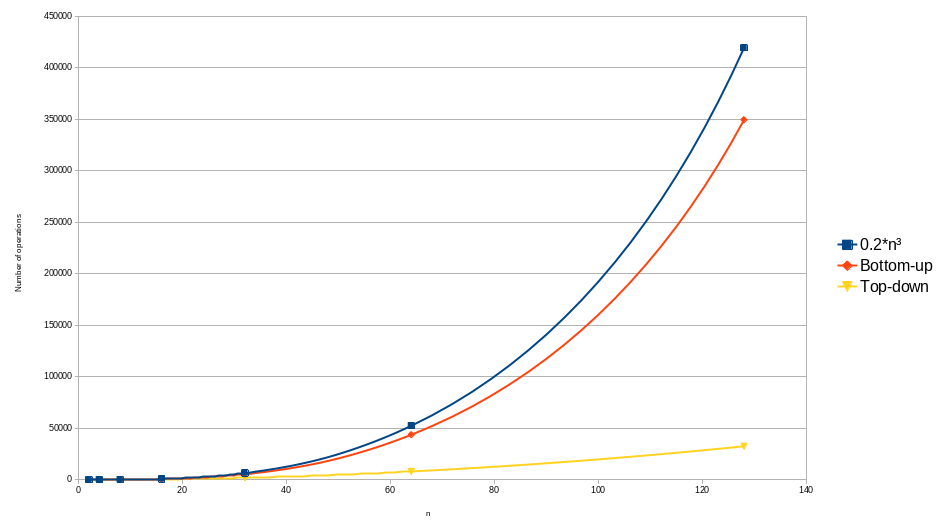
\includegraphics[width=\textwidth]{paren/complexity_paren_lefts_rights}
  
  \caption{Measured number of operations for $\frac n2$ opening followed by
    $\frac n2$ closing, i.e. '(((...)))'\\
    \textit{The naive number of operations is too high to be on
             the graph, or even computed in a reasonable time}}
  
\end{figure*}
\begin{multicols}{2}

As expected, the naive algorithm's number of operations is far higher than the two
other algorithms'. The reason why the top-down version is more efficient than the
bottom-up one is probably that,
given the way it is implemented, it finds a solution very quickly and does not
waste too much time with solutionless recursive calls, while the bottom-up
version computes the parsing of every substring with every production rule no
matter what.

\end{multicols}
\newpage
\begin{figure*}[!htb]
\begin{minipage}{0.48\textwidth}
  \label{fig:plr}
  \centering
  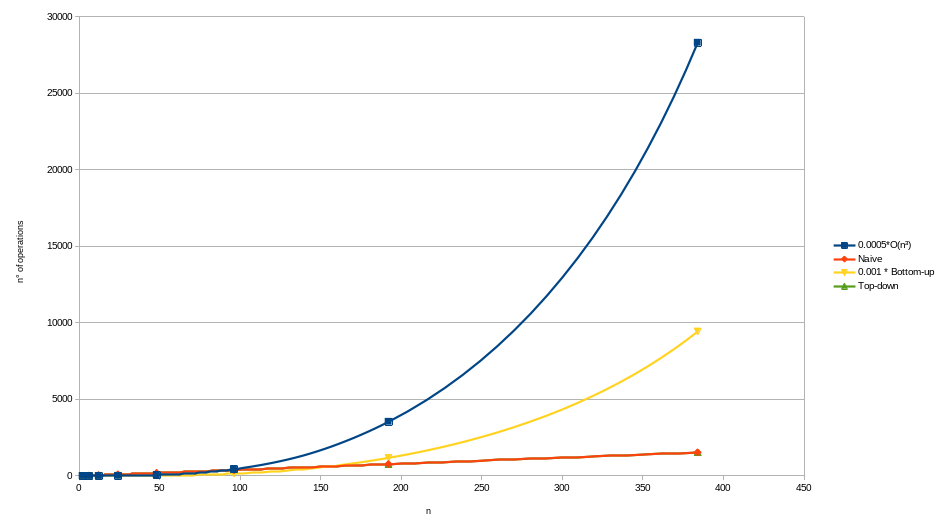
\includegraphics[width=\linewidth]{paren/complexity_paren_left_right}
  \caption{Measured number of operations for $\frac n2$ pairs, i.e. '()()...'}
\end{minipage}\hfill
\begin{minipage}{0.48\textwidth}
  \centering
  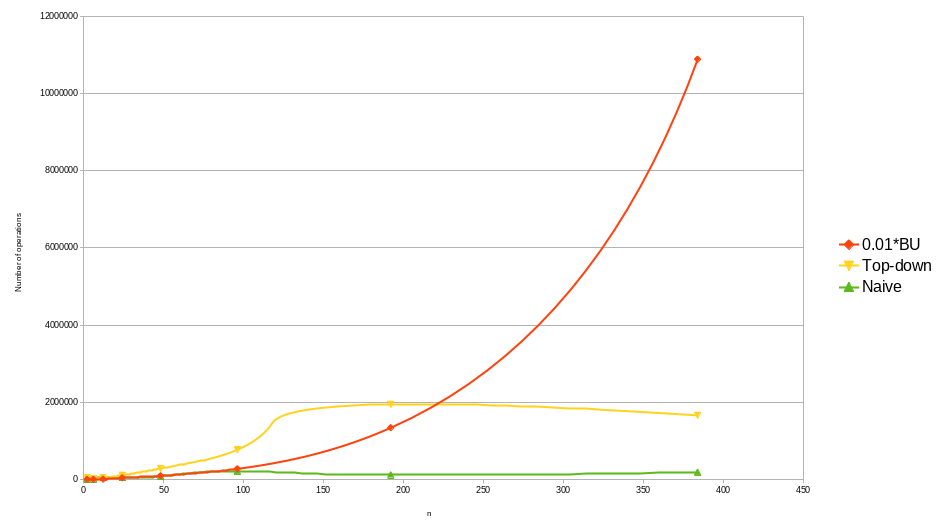
\includegraphics[width=\linewidth]{paren/time_paren_left_right}
  \caption{Measured execution time for $\frac n2$ pairs, i.e. '()()...'}
\end{minipage}
\end{figure*}

\begin{multicols}{2}


Here, both the naive and the top-down variants seem to show a linear number of
operations, whilst the bottom-up variant has a quadratic behaviour. This again
probably comes from the fact that the bottom-up variant performs the parsing for
every possible substring while the others algorithms stop at the first positive recursive call.

Recall that, both for the naive and the top-down DP algorithms, if the two first recursive calls (i.e.
$k=i+1$) are positive each time, the cost is linear, since the recursion is
equivalent to a basic for loop over the string. We hence are in the best
possible case for the top-down algorithms.

It is interesting to note that, in terms of effective computation time, the
naive version is slightly faster than the top-down one. This is probably because
it has no additional table management to perform.

\end{multicols}
\newpage
\begin{figure*}[h]
  \label{fig:plr}
  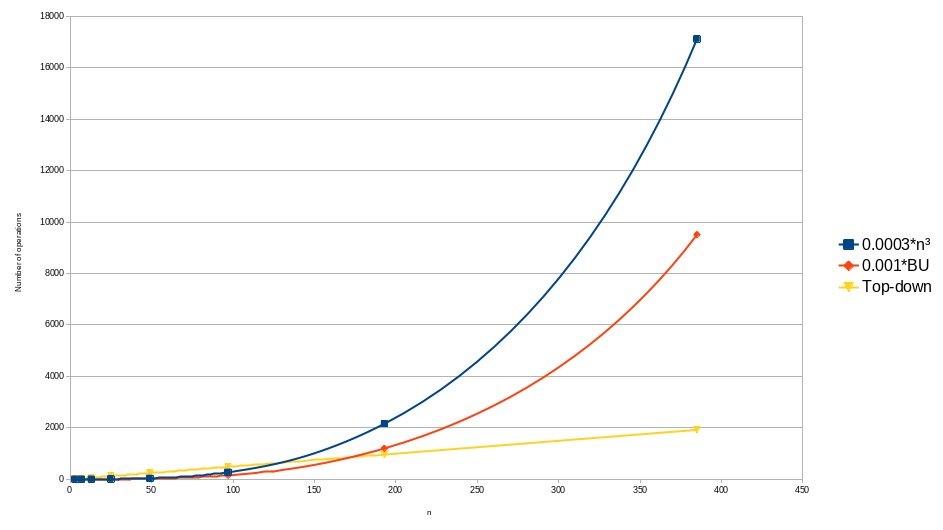
\includegraphics[width=\textwidth]{paren/complexity_closing_paren_left_right}
  \caption{Measured number of operations for closing parenthesis then $\frac n2-1$ pairs, i.e. ')()()...'\\
    \textit{The naive number of operations is too high to be on the graph}}
\end{figure*}
\begin{multicols}{2}

Here, we obtain the same behavior as in the \\``$\frac n2$ opening followed by $\frac n2$
closing, i.e. (((...)))'' case, but with an overall smaller number of
operations. The top-down DP version's number of operations also seems close to
linear again but is probably not, else the naive version's number of operations
would also be close to linear.

\newpage
\subsubsection{Stupid grammar}
The grammar used for the next tests does not generate any word (i.e.
$L(G)=\emptyset$) but the parsing algorithms can still be applied to it. Here is how it looks:
\begin{align*}
  S&\rightarrow ST|TS\\
  T&\rightarrow a
\end{align*}
% \paragraph{tests}\mbox{}\\

The algorithms will end up halting because, even though following the rules until
getting a string is infinite (since we always end up with nonterminal symbols),
the running times depend on the input string. If the algorithms didn't end up halting, we would not be able to guarantee a
$O(n^3)$ running time with dynamic programming anyway.

\end{multicols}
\begin{figure*}[h]
  \label{fig:plr}
  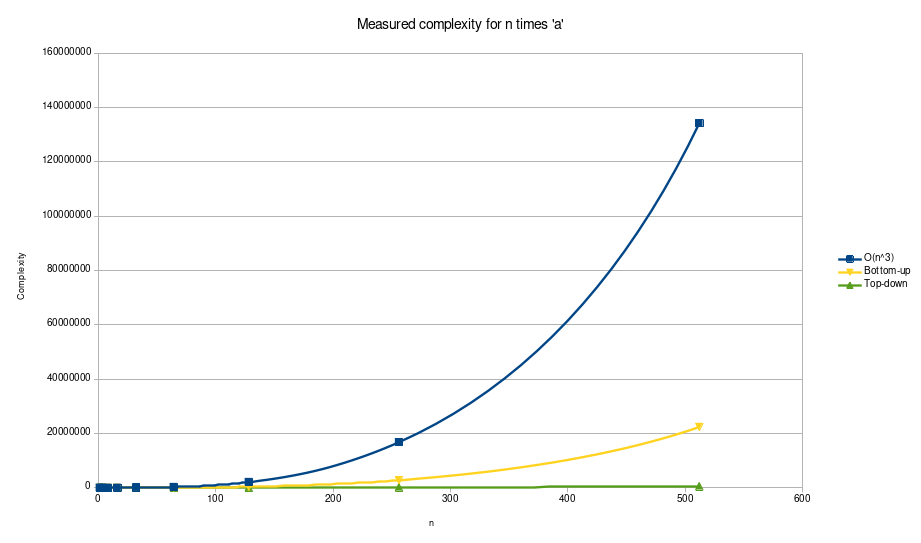
\includegraphics[width=\textwidth]{as/as}
  \caption{Measured number of operations for several a's, i.e. 'aa...'\\
    \textit{The naive number of operations is too high to be on
      the graph}}
\end{figure*}

\begin{multicols}{2}
The reason why the top-down version is faster than the bottom-up one is probably
that all the possible
computations are quickly stored in the table, which then allows to stop using
recursive calls, whilst the bottom-up version does not have that kind of ``memory''.


\newpage
\section{Linear grammars}
This part focuses on how to parse linear grammars (see \ref{sec:linear}), using the
previously detailed bottom-up CYK algorithm.

\subsection{Solution 1: Turn the grammar into Chomsky normal form}
This is the easy solution: Transform each rule of the grammar that does not
match CNF into two CNF rule:
\begin{align*}
  A\rightarrow B\alpha&\equiv A\rightarrow BC,C\rightarrow\alpha \\
  A\rightarrow\alpha B&\equiv A\rightarrow CB,C\rightarrow\alpha
\end{align*}
Obviously, rules of form $A\rightarrow \alpha$ do not have to be changed.

Since each initial rule generates at most 2 CNF rules, the size of the generated
CNF grammar is $O(2|G|)=O(|G|)$, $|G|$ being initial grammar's size. The
transformation time complexity is $O(|G|) = O(1)$.
Since the CYK algorithm has a $O(n^3)$ time complexity, the total parsing time complexity is $O(1)+O(n^3)=O(n^3)$.

\subsection{Solution 2: Adapt the CYK algorithm}
Turning a linear grammar into CNF, then applying the CYK algorithm gives the
same asymptotic time complexity as directly
applying the CYK algorithm to an existing CNF grammar, but we can do better.

It is possible to adapt the CYK algorithm to parse linear grammars, changing the
way the global table is updated. The idea is that instead of testing every
possible string partitions, we check partitions of sizes $(1, n-1)$ for rules of the
form $A\rightarrow\alpha B$ and partitions of sizes $(n-1,1)$ for rules of the form $A\rightarrow B\alpha$.
% Formally, in the bottom-up version, the table is now filled as follows:\\
% Let $G=(N,\Sigma,P,S)$, and $t$ a global three-dimensional table, $s$ the parsed string and $n = |s|$.\\
% $t[i,j]=\displaystyle\bigcup_{A\in N}\{A|A\rightarrow s[i]t[i-1,j+1]\in P\newline\lor A \rightarrow t[i-1,j]s[i+j-1] \in P\}$\\for $i\in [1,n],j \in [1, n-i+1]$\\
% % TODO: explain that the first line is filled like with the CYK algorithm
% If $S \in t[1,n]\quad s \in L(G)$, else $s \notin L(G)$.
Since we only have two possible configurations for each nonterminal rule
(instead of $n$ in the CNF case), there is one less loop bounded by $n$, compared
to the CYK algorithm adapted for CNFs. Therefore,
$T(n)=O(n^2|G|)=O(n^2)<O(n^3)$. It is hence worth it to adapt the CYK algorithm
instead of turning $G$ into CNF.

\newpage
\subsection{Empirical measurements}
It is interesting to compare the two previously presented methods to check that both follow the expected behavior.

\subsubsection{abc}
The grammar used for the next tests only accepts strings of form $a^kb^lc^k\ \forall k\in \mathbb{N}\ \forall l\in\mathbb{N}\backslash 0$:\\
\begin{align*}
  G&=(N,\Sigma,P,A)\\
  P&=\
  \left\{ \begin{array}{l}
    S\rightarrow Ac\\
    S\rightarrow b\\
    A\rightarrow aS\\
    A\rightarrow aB\\
    B\rightarrow bS
  \end{array}\right\}
\end{align*}

\end{multicols}
\textbf{Inputs from $L(G)$}\\
Here are the measured numbers of operations for strings from $L(G)$.\\

\begin{figure*}[h]
  \label{fig:plr}
  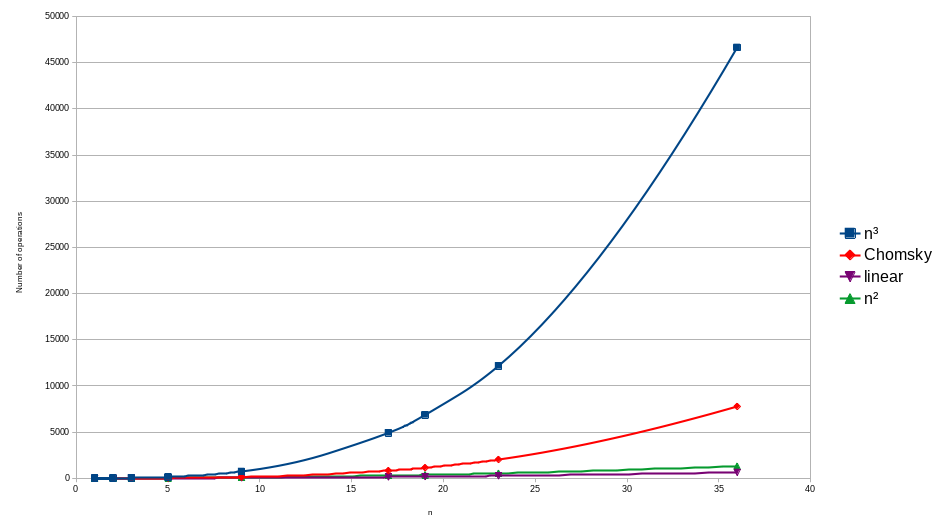
\includegraphics[width=\textwidth]{linear/complexity_as_bs_cs}
  \caption{Measured number of operations for $a^kb^lc^k$}
\end{figure*}

\begin{multicols}{2}
% As expected, the adapted CYK algorithm's is of execution time $O(n^2)$ for the given inputs, while
% turning $G$ into a CNF grammar, and then executing the CYK algorithm on the new
% CNF grammar is of execution time $O(n^3)$.
As expected, the adapted CYK algorithm seems more efficient than turning $G$ into a
CNF grammar, and then executing the CYK algorithm:
\\\\\\
\begin{itemize}
\item The adapted CYK algorithm shows a $O(n^2)$ number of operations
\item Turning $G$ into a CNF grammar, then executing the CYK algorithm shows a
  $O(n^3)$ number of operations
\end{itemize}

\end{multicols}
\newpage
\textbf{Inputs not from $L(G)$}\\
Here are the measured numbers of operations for random strings not from $L(G)$, i.e. $\{\alpha=(a+b+c)^n|\alpha\notin L(G)\}$.\\

\begin{figure*}[h]
  \label{fig:plr}
  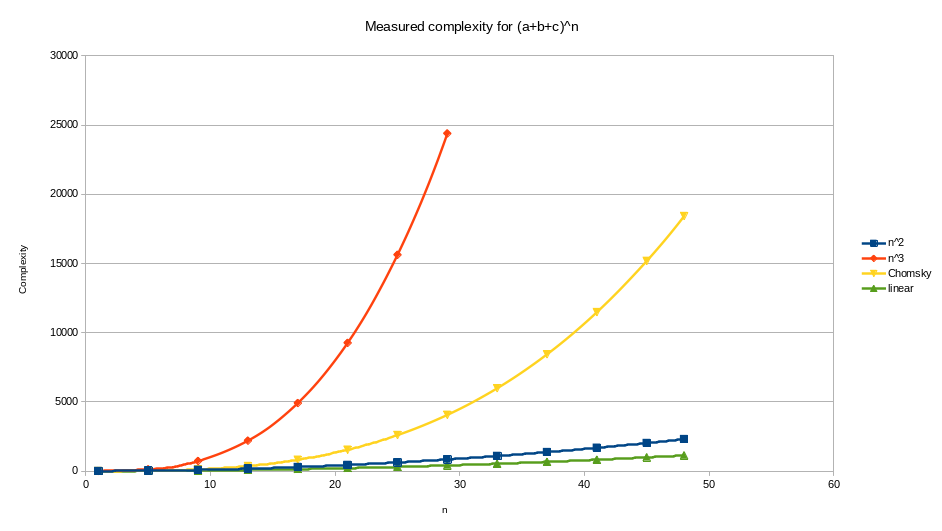
\includegraphics[width=\textwidth]{linear/complexity_random_abc}
  \caption{measured numbers of operations for $(a+b+c)^n$}
\end{figure*}


\begin{multicols}{2}
With wrong inputs, The measured numbers of operations keep the same
behavior. This confirms that it seems more efficient to adapt the CYK algorithm
to linear grammars, instead of translating linear grammars into CNF.

\end{multicols}
\end{document}